\documentclass{standalone}
\usepackage{tikz}
\usetikzlibrary{patterns, positioning}

\begin{document}
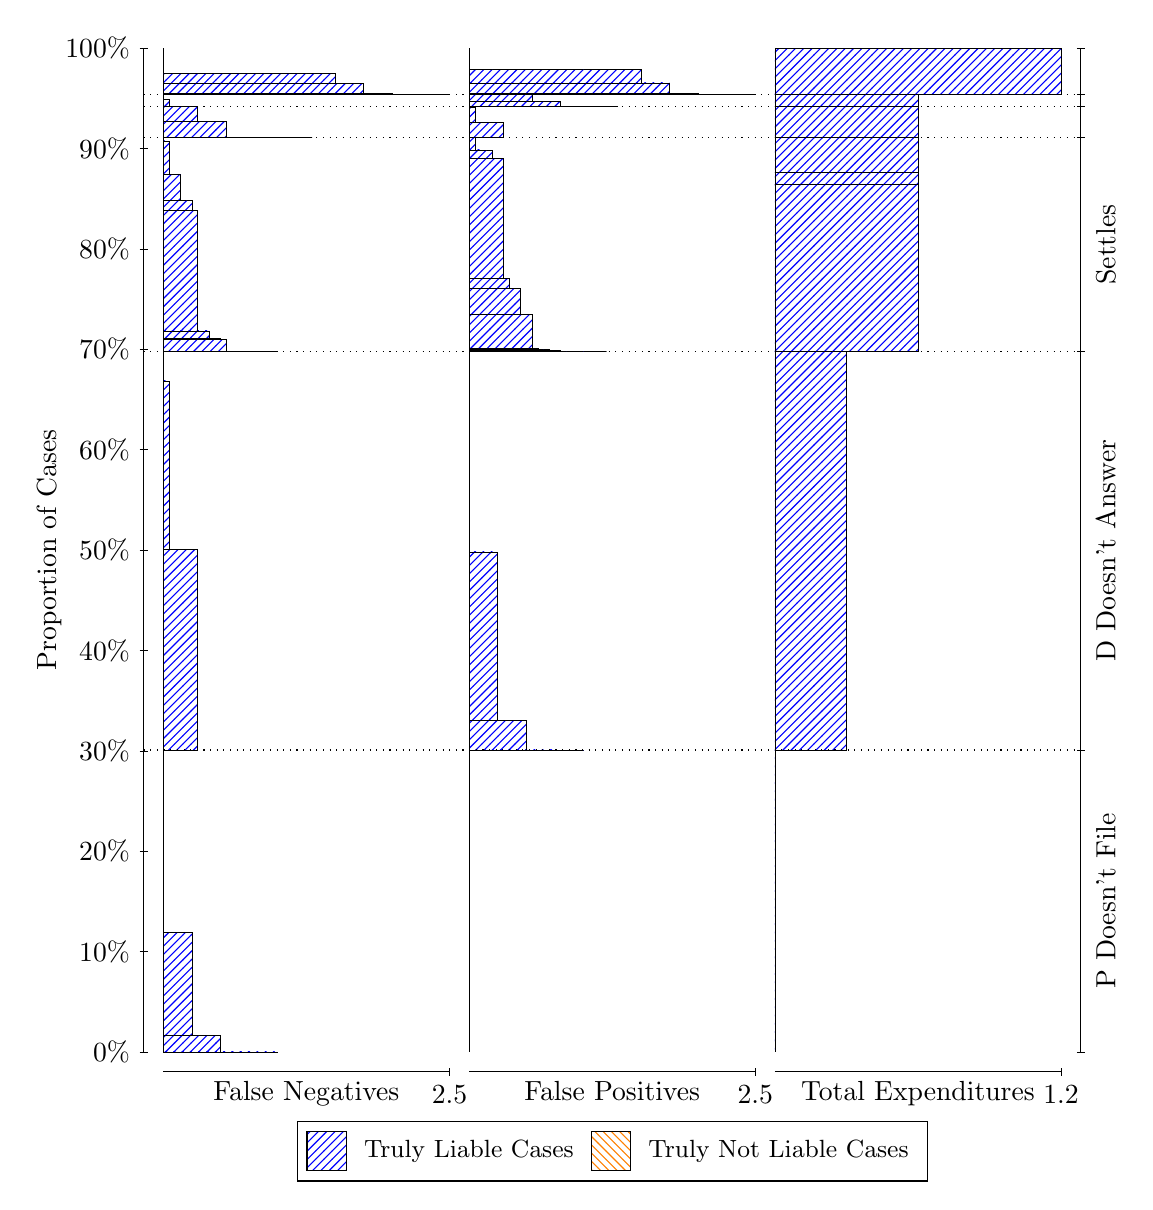
\begin{tikzpicture}
\draw[black, very thin] (1.5,1.75) -- (1.5,14.5);
\node[rotate=90, anchor=center] at (0.3, 8.125) {Proportion of Cases};
\draw[black, very thin] (1.45,1.75) -- (1.55,1.75);
\node[anchor=east] at (1.45, 1.75) {0\%};
\draw[black, very thin] (1.45,3.025) -- (1.55,3.025);
\node[anchor=east] at (1.45, 3.025) {10\%};
\draw[black, very thin] (1.45,4.3) -- (1.55,4.3);
\node[anchor=east] at (1.45, 4.3) {20\%};
\draw[black, very thin] (1.45,5.575) -- (1.55,5.575);
\node[anchor=east] at (1.45, 5.575) {30\%};
\draw[black, very thin] (1.45,6.85) -- (1.55,6.85);
\node[anchor=east] at (1.45, 6.85) {40\%};
\draw[black, very thin] (1.45,8.125) -- (1.55,8.125);
\node[anchor=east] at (1.45, 8.125) {50\%};
\draw[black, very thin] (1.45,9.4) -- (1.55,9.4);
\node[anchor=east] at (1.45, 9.4) {60\%};
\draw[black, very thin] (1.45,10.675) -- (1.55,10.675);
\node[anchor=east] at (1.45, 10.675) {70\%};
\draw[black, very thin] (1.45,11.95) -- (1.55,11.95);
\node[anchor=east] at (1.45, 11.95) {80\%};
\draw[black, very thin] (1.45,13.225) -- (1.55,13.225);
\node[anchor=east] at (1.45, 13.225) {90\%};
\draw[black, very thin] (1.45,14.5) -- (1.55,14.5);
\node[anchor=east] at (1.45, 14.5) {100\%};

\draw[black, very thin] (13.4,1.75) -- (13.4,14.5);
\draw[black, very thin] (13.35,1.75) -- (13.45,1.75);
\node[anchor=west] at (13.35, 1.75) {};
\draw[black, very thin] (13.35,5.5846) -- (13.45,5.5846);
\node[anchor=west] at (13.35, 5.5846) {};
\draw[black, very thin] (13.35,10.647) -- (13.45,10.647);
\node[anchor=west] at (13.35, 10.647) {};
\draw[black, very thin] (13.35,13.363) -- (13.45,13.363);
\node[anchor=west] at (13.35, 13.363) {};
\draw[black, very thin] (13.35,13.754) -- (13.45,13.754);
\node[anchor=west] at (13.35, 13.754) {};
\draw[black, very thin] (13.35,13.91) -- (13.45,13.91);
\node[anchor=west] at (13.35, 13.91) {};
\draw[black, very thin] (13.35,14.5) -- (13.45,14.5);
\node[anchor=west] at (13.35, 14.5) {};

\draw[black, very thin, pattern color=blue, pattern=north east lines] (1.75,1.75) rectangle (3.2033,1.75);
\draw[black, very thin, pattern color=blue, pattern=north east lines] (1.75,1.75) rectangle (2.84,1.7518);
\draw[black, very thin, pattern color=blue, pattern=north east lines] (1.75,1.7518) rectangle (2.4767,1.9632);
\draw[black, very thin, pattern color=blue, pattern=north east lines] (1.75,1.9632) rectangle (2.1133,3.2683);
\draw[black, very thin, pattern color=orange, pattern=north west lines] (1.75,3.2683) rectangle (1.75,3.2683);
\draw[black, very thin, pattern color=blue, pattern=north east lines] (1.75,3.2683) rectangle (1.75,5.5846);
\draw[black, very thin, pattern color=blue, pattern=north east lines] (1.75,5.5846) rectangle (2.186,8.1304);
\draw[black, very thin, pattern color=blue, pattern=north east lines] (1.75,8.1304) rectangle (1.8227,10.274);
\draw[black, very thin, pattern color=orange, pattern=north west lines] (1.75,10.274) rectangle (1.75,10.274);
\draw[black, very thin, pattern color=blue, pattern=north east lines] (1.75,10.274) rectangle (1.75,10.647);
\draw[black, very thin, pattern color=blue, pattern=north east lines] (1.75,10.647) rectangle (3.2033,10.647);
\draw[black, very thin, pattern color=blue, pattern=north east lines] (1.75,10.647) rectangle (3.058,10.647);
\draw[black, very thin, pattern color=blue, pattern=north east lines] (1.75,10.647) rectangle (2.9127,10.647);
\draw[black, very thin, pattern color=blue, pattern=north east lines] (1.75,10.647) rectangle (2.84,10.647);
\draw[black, very thin, pattern color=blue, pattern=north east lines] (1.75,10.647) rectangle (2.7673,10.647);
\draw[black, very thin, pattern color=blue, pattern=north east lines] (1.75,10.647) rectangle (2.6947,10.647);
\draw[black, very thin, pattern color=blue, pattern=north east lines] (1.75,10.647) rectangle (2.622,10.647);
\draw[black, very thin, pattern color=blue, pattern=north east lines] (1.75,10.647) rectangle (2.5493,10.803);
\draw[black, very thin, pattern color=blue, pattern=north east lines] (1.75,10.803) rectangle (2.4767,10.81);
\draw[black, very thin, pattern color=blue, pattern=north east lines] (1.75,10.81) rectangle (2.404,10.81);
\draw[black, very thin, pattern color=blue, pattern=north east lines] (1.75,10.81) rectangle (2.3313,10.907);
\draw[black, very thin, pattern color=blue, pattern=north east lines] (1.75,10.907) rectangle (2.3313,10.907);
\draw[black, very thin, pattern color=blue, pattern=north east lines] (1.75,10.907) rectangle (2.2587,10.907);
\draw[black, very thin, pattern color=blue, pattern=north east lines] (1.75,10.907) rectangle (2.186,12.437);
\draw[black, very thin, pattern color=blue, pattern=north east lines] (1.75,12.437) rectangle (2.1133,12.564);
\draw[black, very thin, pattern color=blue, pattern=north east lines] (1.75,12.564) rectangle (2.0407,12.564);
\draw[black, very thin, pattern color=blue, pattern=north east lines] (1.75,12.564) rectangle (1.968,12.891);
\draw[black, very thin, pattern color=blue, pattern=north east lines] (1.75,12.891) rectangle (1.968,12.891);
\draw[black, very thin, pattern color=blue, pattern=north east lines] (1.75,12.891) rectangle (1.8953,12.891);
\draw[black, very thin, pattern color=blue, pattern=north east lines] (1.75,12.891) rectangle (1.8227,13.321);
\draw[black, very thin, pattern color=orange, pattern=north west lines] (1.75,13.321) rectangle (1.75,13.321);
\draw[black, very thin, pattern color=blue, pattern=north east lines] (1.75,13.321) rectangle (1.75,13.363);
\draw[black, very thin, pattern color=blue, pattern=north east lines] (1.75,13.363) rectangle (3.6393,13.363);
\draw[black, very thin, pattern color=blue, pattern=north east lines] (1.75,13.363) rectangle (3.276,13.363);
\draw[black, very thin, pattern color=blue, pattern=north east lines] (1.75,13.363) rectangle (2.9127,13.367);
\draw[black, very thin, pattern color=blue, pattern=north east lines] (1.75,13.367) rectangle (2.5493,13.567);
\draw[black, very thin, pattern color=blue, pattern=north east lines] (1.75,13.567) rectangle (2.186,13.754);
\draw[black, very thin, pattern color=orange, pattern=north west lines] (1.75,13.754) rectangle (1.75,13.754);
\draw[black, very thin, pattern color=blue, pattern=north east lines] (1.75,13.754) rectangle (2.186,13.756);
\draw[black, very thin, pattern color=blue, pattern=north east lines] (1.75,13.756) rectangle (1.8227,13.844);
\draw[black, very thin, pattern color=orange, pattern=north west lines] (1.75,13.844) rectangle (1.75,13.844);
\draw[black, very thin, pattern color=blue, pattern=north east lines] (1.75,13.844) rectangle (1.75,13.91);
\draw[black, very thin, pattern color=blue, pattern=north east lines] (1.75,13.91) rectangle (5.3833,13.91);
\draw[black, very thin, pattern color=blue, pattern=north east lines] (1.75,13.91) rectangle (5.02,13.91);
\draw[black, very thin, pattern color=blue, pattern=north east lines] (1.75,13.91) rectangle (4.6567,13.919);
\draw[black, very thin, pattern color=blue, pattern=north east lines] (1.75,13.919) rectangle (4.2933,14.054);
\draw[black, very thin, pattern color=blue, pattern=north east lines] (1.75,14.054) rectangle (3.93,14.179);
\draw[black, very thin, pattern color=blue, pattern=north east lines] (1.75,14.179) rectangle (3.5667,14.179);
\draw[black, very thin, pattern color=blue, pattern=north east lines] (1.75,14.179) rectangle (3.2033,14.179);
\draw[black, very thin, pattern color=blue, pattern=north east lines] (1.75,14.179) rectangle (2.404,14.179);
\draw[black, very thin, pattern color=blue, pattern=north east lines] (1.75,14.179) rectangle (2.0407,14.179);
\draw[black, very thin, pattern color=orange, pattern=north west lines] (1.75,14.179) rectangle (1.75,14.179);
\draw[black, very thin, pattern color=blue, pattern=north east lines] (1.75,14.179) rectangle (1.75,14.5);
\draw[black, very thin, pattern color=orange, pattern=north west lines] (5.6333,1.75) rectangle (5.6333,1.75);
\draw[black, very thin, pattern color=blue, pattern=north east lines] (5.6333,1.75) rectangle (5.6333,5.5846);
\draw[black, very thin, pattern color=orange, pattern=north west lines] (5.6333,5.5846) rectangle (7.0867,5.5846);
\draw[black, very thin, pattern color=blue, pattern=north east lines] (5.6333,5.5846) rectangle (7.0867,5.5846);
\draw[black, very thin, pattern color=blue, pattern=north east lines] (5.6333,5.5846) rectangle (6.7233,5.5863);
\draw[black, very thin, pattern color=blue, pattern=north east lines] (5.6333,5.5863) rectangle (6.36,5.9573);
\draw[black, very thin, pattern color=blue, pattern=north east lines] (5.6333,5.9573) rectangle (5.9967,8.1007);
\draw[black, very thin, pattern color=blue, pattern=north east lines] (5.6333,8.1007) rectangle (5.6333,10.647);
\draw[black, very thin, pattern color=orange, pattern=north west lines] (5.6333,10.647) rectangle (7.3773,10.647);
\draw[black, very thin, pattern color=blue, pattern=north east lines] (5.6333,10.647) rectangle (7.3773,10.647);
\draw[black, very thin, pattern color=orange, pattern=north west lines] (5.6333,10.647) rectangle (7.232,10.647);
\draw[black, very thin, pattern color=blue, pattern=north east lines] (5.6333,10.647) rectangle (7.232,10.647);
\draw[black, very thin, pattern color=orange, pattern=north west lines] (5.6333,10.647) rectangle (7.0867,10.647);
\draw[black, very thin, pattern color=blue, pattern=north east lines] (5.6333,10.647) rectangle (7.0867,10.647);
\draw[black, very thin, pattern color=blue, pattern=north east lines] (5.6333,10.647) rectangle (7.014,10.647);
\draw[black, very thin, pattern color=orange, pattern=north west lines] (5.6333,10.647) rectangle (6.9413,10.647);
\draw[black, very thin, pattern color=blue, pattern=north east lines] (5.6333,10.647) rectangle (6.9413,10.647);
\draw[black, very thin, pattern color=blue, pattern=north east lines] (5.6333,10.647) rectangle (6.8687,10.647);
\draw[black, very thin, pattern color=orange, pattern=north west lines] (5.6333,10.647) rectangle (6.796,10.647);
\draw[black, very thin, pattern color=blue, pattern=north east lines] (5.6333,10.647) rectangle (6.796,10.657);
\draw[black, very thin, pattern color=blue, pattern=north east lines] (5.6333,10.657) rectangle (6.7233,10.657);
\draw[black, very thin, pattern color=orange, pattern=north west lines] (5.6333,10.657) rectangle (6.6507,10.657);
\draw[black, very thin, pattern color=blue, pattern=north east lines] (5.6333,10.657) rectangle (6.6507,10.676);
\draw[black, very thin, pattern color=blue, pattern=north east lines] (5.6333,10.676) rectangle (6.578,10.676);
\draw[black, very thin, pattern color=blue, pattern=north east lines] (5.6333,10.676) rectangle (6.5053,10.676);
\draw[black, very thin, pattern color=orange, pattern=north west lines] (5.6333,10.676) rectangle (6.5053,10.676);
\draw[black, very thin, pattern color=blue, pattern=north east lines] (5.6333,10.676) rectangle (6.5053,10.689);
\draw[black, very thin, pattern color=blue, pattern=north east lines] (5.6333,10.689) rectangle (6.4327,11.118);
\draw[black, very thin, pattern color=blue, pattern=north east lines] (5.6333,11.118) rectangle (6.36,11.118);
\draw[black, very thin, pattern color=blue, pattern=north east lines] (5.6333,11.118) rectangle (6.2873,11.446);
\draw[black, very thin, pattern color=blue, pattern=north east lines] (5.6333,11.446) rectangle (6.2147,11.446);
\draw[black, very thin, pattern color=blue, pattern=north east lines] (5.6333,11.446) rectangle (6.142,11.446);
\draw[black, very thin, pattern color=blue, pattern=north east lines] (5.6333,11.446) rectangle (6.142,11.573);
\draw[black, very thin, pattern color=blue, pattern=north east lines] (5.6333,11.573) rectangle (6.0693,13.103);
\draw[black, very thin, pattern color=blue, pattern=north east lines] (5.6333,13.103) rectangle (5.9967,13.103);
\draw[black, very thin, pattern color=blue, pattern=north east lines] (5.6333,13.103) rectangle (5.924,13.2);
\draw[black, very thin, pattern color=blue, pattern=north east lines] (5.6333,13.2) rectangle (5.8513,13.2);
\draw[black, very thin, pattern color=blue, pattern=north east lines] (5.6333,13.2) rectangle (5.7787,13.2);
\draw[black, very thin, pattern color=blue, pattern=north east lines] (5.6333,13.2) rectangle (5.7787,13.207);
\draw[black, very thin, pattern color=blue, pattern=north east lines] (5.6333,13.207) rectangle (5.706,13.363);
\draw[black, very thin, pattern color=blue, pattern=north east lines] (5.6333,13.363) rectangle (5.6333,13.363);
\draw[black, very thin, pattern color=orange, pattern=north west lines] (5.6333,13.363) rectangle (6.0693,13.363);
\draw[black, very thin, pattern color=blue, pattern=north east lines] (5.6333,13.363) rectangle (6.0693,13.551);
\draw[black, very thin, pattern color=blue, pattern=north east lines] (5.6333,13.551) rectangle (5.706,13.751);
\draw[black, very thin, pattern color=blue, pattern=north east lines] (5.6333,13.751) rectangle (5.6333,13.754);
\draw[black, very thin, pattern color=orange, pattern=north west lines] (5.6333,13.754) rectangle (7.5227,13.754);
\draw[black, very thin, pattern color=blue, pattern=north east lines] (5.6333,13.754) rectangle (7.5227,13.754);
\draw[black, very thin, pattern color=blue, pattern=north east lines] (5.6333,13.754) rectangle (7.1593,13.755);
\draw[black, very thin, pattern color=blue, pattern=north east lines] (5.6333,13.755) rectangle (6.796,13.821);
\draw[black, very thin, pattern color=blue, pattern=north east lines] (5.6333,13.821) rectangle (6.4327,13.908);
\draw[black, very thin, pattern color=blue, pattern=north east lines] (5.6333,13.908) rectangle (6.0693,13.91);
\draw[black, very thin, pattern color=orange, pattern=north west lines] (5.6333,13.91) rectangle (9.2667,13.91);
\draw[black, very thin, pattern color=blue, pattern=north east lines] (5.6333,13.91) rectangle (9.2667,13.91);
\draw[black, very thin, pattern color=orange, pattern=north west lines] (5.6333,13.91) rectangle (8.9033,13.91);
\draw[black, very thin, pattern color=blue, pattern=north east lines] (5.6333,13.91) rectangle (8.9033,13.91);
\draw[black, very thin, pattern color=orange, pattern=north west lines] (5.6333,13.91) rectangle (8.54,13.91);
\draw[black, very thin, pattern color=blue, pattern=north east lines] (5.6333,13.91) rectangle (8.54,13.919);
\draw[black, very thin, pattern color=orange, pattern=north west lines] (5.6333,13.919) rectangle (8.1767,13.919);
\draw[black, very thin, pattern color=blue, pattern=north east lines] (5.6333,13.919) rectangle (8.1767,14.056);
\draw[black, very thin, pattern color=blue, pattern=north east lines] (5.6333,14.056) rectangle (7.8133,14.229);
\draw[black, very thin, pattern color=blue, pattern=north east lines] (5.6333,14.229) rectangle (7.45,14.23);
\draw[black, very thin, pattern color=blue, pattern=north east lines] (5.6333,14.23) rectangle (7.0867,14.23);
\draw[black, very thin, pattern color=blue, pattern=north east lines] (5.6333,14.23) rectangle (6.7233,14.23);
\draw[black, very thin, pattern color=orange, pattern=north west lines] (5.6333,14.23) rectangle (5.924,14.23);
\draw[black, very thin, pattern color=blue, pattern=north east lines] (5.6333,14.23) rectangle (5.924,14.23);
\draw[black, very thin, pattern color=orange, pattern=north west lines] (5.6333,14.23) rectangle (5.6333,14.23);
\draw[black, very thin, pattern color=blue, pattern=north east lines] (5.6333,14.23) rectangle (5.6333,14.5);
\draw[black, very thin, pattern color=orange, pattern=north west lines] (9.5167,1.75) rectangle (9.5167,1.75);
\draw[black, very thin, pattern color=blue, pattern=north east lines] (9.5167,1.75) rectangle (9.5167,5.5846);
\draw[black, very thin, pattern color=orange, pattern=north west lines] (9.5167,5.5846) rectangle (10.425,5.5846);
\draw[black, very thin, pattern color=blue, pattern=north east lines] (9.5167,5.5846) rectangle (10.425,10.647);
\draw[black, very thin, pattern color=orange, pattern=north west lines] (9.5167,10.647) rectangle (11.333,10.647);
\draw[black, very thin, pattern color=blue, pattern=north east lines] (9.5167,10.647) rectangle (11.333,12.773);
\draw[black, very thin, pattern color=orange, pattern=north west lines] (9.5167,12.773) rectangle (11.333,12.773);
\draw[black, very thin, pattern color=blue, pattern=north east lines] (9.5167,12.773) rectangle (11.333,12.92);
\draw[black, very thin, pattern color=orange, pattern=north west lines] (9.5167,12.92) rectangle (11.333,12.92);
\draw[black, very thin, pattern color=blue, pattern=north east lines] (9.5167,12.92) rectangle (11.333,13.363);
\draw[black, very thin, pattern color=orange, pattern=north west lines] (9.5167,13.363) rectangle (11.333,13.363);
\draw[black, very thin, pattern color=blue, pattern=north east lines] (9.5167,13.363) rectangle (11.333,13.754);
\draw[black, very thin, pattern color=orange, pattern=north west lines] (9.5167,13.754) rectangle (11.333,13.754);
\draw[black, very thin, pattern color=blue, pattern=north east lines] (9.5167,13.754) rectangle (11.333,13.91);
\draw[black, very thin, pattern color=orange, pattern=north west lines] (9.5167,13.91) rectangle (13.15,13.91);
\draw[black, very thin, pattern color=blue, pattern=north east lines] (9.5167,13.91) rectangle (13.15,14.5);
\draw[black, dotted] (1.5,5.5846) -- (13.4,5.5846);
\draw[black, dotted] (1.5,10.647) -- (13.4,10.647);
\draw[black, dotted] (1.5,13.363) -- (13.4,13.363);
\draw[black, dotted] (1.5,13.754) -- (13.4,13.754);
\draw[black, dotted] (1.5,13.91) -- (13.4,13.91);
\draw[black, very thin] (1.75,1.5) -- (5.3833,1.5);
\node[anchor=north] at (3.5667, 1.5) {False Negatives};
\draw[black, very thin] (5.3833,1.45) -- (5.3833,1.55);
\node[anchor=north] at (5.3833, 1.45) {2.5};

\draw[black, very thin] (5.6333,1.5) -- (9.2667,1.5);
\node[anchor=north] at (7.45, 1.5) {False Positives};
\draw[black, very thin] (9.2667,1.45) -- (9.2667,1.55);
\node[anchor=north] at (9.2667, 1.45) {2.5};

\draw[black, very thin] (9.5167,1.5) -- (13.15,1.5);
\node[anchor=north] at (11.333, 1.5) {Total Expenditures};
\draw[black, very thin] (13.15,1.45) -- (13.15,1.55);
\node[anchor=north] at (13.15, 1.45) {1.2};

\node[black, centered, rotate=90] at (13.72, 3.6673) {P Doesn't File};
\node[black, centered, rotate=90] at (13.72, 8.1156) {D Doesn't Answer};
\node[black, centered, rotate=90] at (13.72, 12.005) {Settles};




\draw (7.449999999999999,1.5) node[draw=none] (baseCoordinate) {};
\begin{scope}[align=center]
        \matrix[scale=0.5, draw=black, below=0.5cm of baseCoordinate, nodes={draw}, column sep=0.1cm]{
            \node[rectangle, draw, minimum width=0.5cm, minimum height=0.5cm, pattern=north east lines, pattern color=blue] {}; &
            \node[draw=none, font=\small] (B) {Truly Liable Cases}; &
            \node[rectangle, draw, minimum width=0.5cm, minimum height=0.5cm, pattern=north west lines, pattern color=orange] {}; &
            \node[draw=none, font=\small] (B) {Truly Not Liable Cases}; \\
            };
\end{scope}

\end{tikzpicture}
\end{document}